\documentclass[11pt, oneside]{article}   	% use "amsart" instead of "article" for AMSLaTeX format
\usepackage{geometry}                		% See geometry.pdf to learn the layout options. There are lots.
\geometry{letterpaper}                   		% ... or a4paper or a5paper or ... 
%\geometry{landscape}                		% Activate for for rotated page geometry
%\usepackage[parfill]{parskip}    		% Activate to begin paragraphs with an empty line rather than an indent
\usepackage{graphicx}				% Use pdf, png, jpg, or eps� with pdflatex; use eps in DVI mode
								% TeX will automatically convert eps --> pdf in pdflatex		
\usepackage{amssymb}
\usepackage{amsmath}
\usepackage{parskip}
\usepackage{color}
\usepackage{hyperref}

\title{Integrating z*}
%\author{The Author}
%\section{}
%\subsection*{}
\date{}							% Activate to display a given date or no date

\graphicspath{{/Users/telliott_admin/Dropbox/Tex/png/}}
% \begin{center} 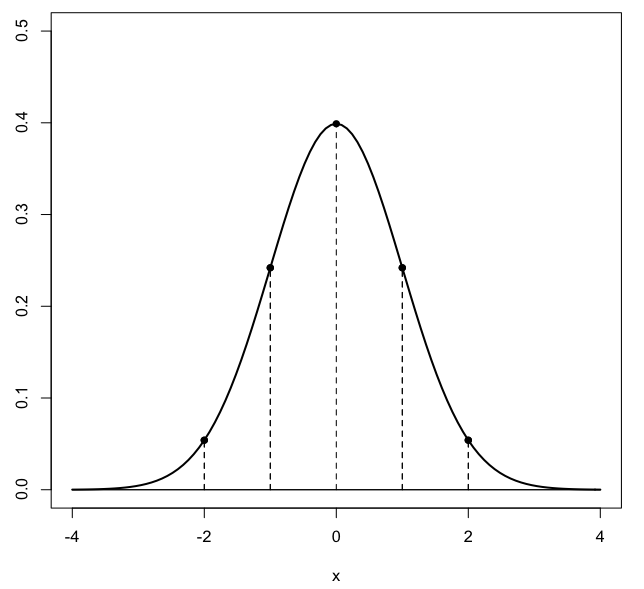
\includegraphics [scale=0.4] {gauss3.png} \end{center}
\begin{document}
\maketitle
\Large
If the contour (curve) of integration $C$ is parametrized in terms of $t$, then
\[ \int_C f(z) \ dz = \int_a^b f[z(t)] \ z'(t) \ dt \]

Let's look at $f(z) = z*$ (note that this function is \emph{not} analytic).

Take our curve to be the circle of radius $2$ centered at the origin, and proceed halfway around, between the endpoints $z = -i \rightarrow i$.

On this curve it is natural to parametrize in terms of $\theta$
\[ z = 2e^{i \theta} \]
we have
\[ dz = 2i e^{i \theta} \ d \theta \]
In radial coordinates the complex conjugate is particularly simple
\[ z* = 2e^{-i\theta} \]
Notice that
\[ zz* = 2e^{i \theta} \ 2e^{-i\theta}  = 4 = |z|^2 \]
For the integral, we have
\[ \int {z*} \ dz = \int 2e^{-i\theta} \ 2i e^{i \theta} \ d \theta \]
\[ = 4 i \int_{-\pi/2}^{\pi/2} d \theta = 4 \pi i \]
A closed contour where we go all the way around would also have a non-zero integral, namely $2 \pi$ times the radius squared, times $i$.

\subsection*{Alternatively}
\[ zz* =  4 \]
\[ \int {z*} \ dz = 4 \int \frac{1}{z} \ dz \]
Again
\[ z = 2e^{i \theta} \]
\[ dz = 2i e^{i \theta} \ d \theta = iz \ d \theta \]
So the integral is just
\[ \int {z*} \ dz = 4 \int \frac{1}{z} \ dz \]
\[ = 4 \int \frac{1}{z} \ iz \ d \theta   \]
\[ = 4 i \int d \theta = 4 \pi i \]

\end{document}  